\section{Data}
\label{sec:data}
Luminous red galaxies are massive galaxies that lack active star formation and considered as one of the highly biased tracers of large scale structure. They are widely targeted in previous galaxy surveys and their clustering and redshift properties are well known. We use the photometric DESI Luminous Red Galaxies (LRG), selected from the imaging surveys \citep{dey2018overview} using color cuts described in the $g$, $r$, $z$, and $W1$ bands \citep[see,][]{zhou2021clustering}, and summarized in Tab. \ref{tab:ts}. The LRG sample are masked for bright stars and foreground bright galaxies and clusters of galaxies\footnote{See \url{https://www.legacysurvey.org/dr9/bitmasks/}}, and then binned into HEALPix \citep{gorski2005healpix} at $\textsc{nside}=256$ to construct the LRG density field, with an average density of $800$ deg$^{-2}$ with a coverage around $14000$ square degrees of the sky, as shown in Fig. \ref{fig:ng}. The density map is accounted for pixel incompleteness using a catalog of random points with the similar cuts and masks as the LRG sample. 

We study the correlation between target density field and potential sources of systematic error, mapped into HEALPix similar to the data. The maps considered in this study are stellar density from \mr{Myers et al. (2022)} from Gaia,  Galactic extinction E[B-V] from \cite{schlegel1998maps}, and other systematics properties including survey depth (galaxy depth in grz and PSF depth in W1) and seeing in grz from DESI imaging. Fig. \ref{fig:pcc} shows the Spearman correlation between galaxy density and imaging properties. 

%Explain the target selection and sample. What bands are used for selection, total area, and maybe their redshift distribution from spectroscopy, and their inferred halo bias. Bitmasks applied based on . SV3 LRG Selection with 800 per sq. deg. Target selection of DESI LRGs is presented in XXX. The selection uses imaging in XXX optical and YY infrared bands (see, e.g., ZZZ). Density of DESI LRGs in deg$^{-2}$ is shown in Fig. \ref{fig:lrgdens}.

\begin{figure}
    \centering
    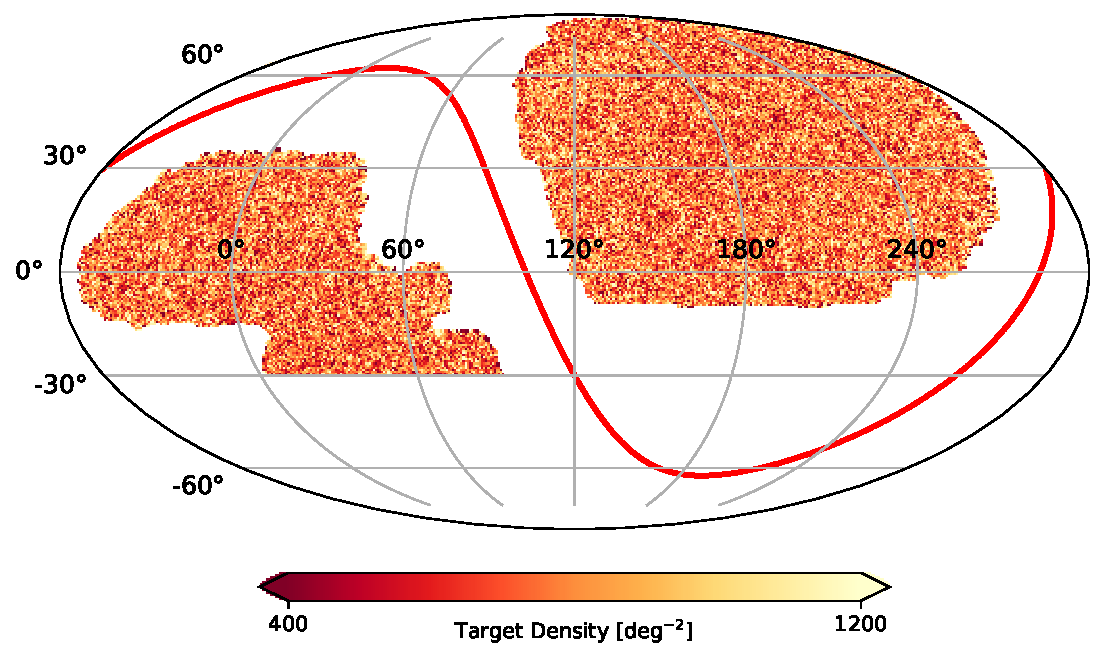
\includegraphics[width=0.45\textwidth]{figures/lrgdens.pdf}
    \caption{Observed density field of DESI Luminous Red Galaxies DR9 in deg$^{-2}$.}
    \label{fig:ng}
\end{figure}

Fig. \ref{fig:nz} shows the redshift distribution of LRGs and the halo bias as a function of redshift \mr{CITE Zhou et al for the bias model}. 
\begin{figure}
    \centering
    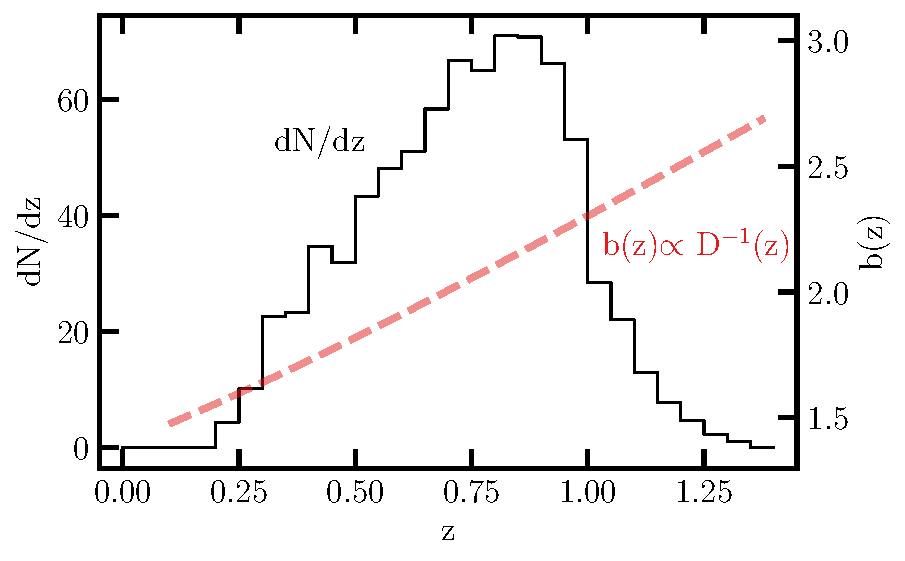
\includegraphics[width=0.45\textwidth]{figures/nz_lrg.pdf}
    \caption{Redshift distribution and linear bias of the DESI Luminous Red Galaxies.}
    \label{fig:nz}
\end{figure}


\begin{figure}
    \centering
    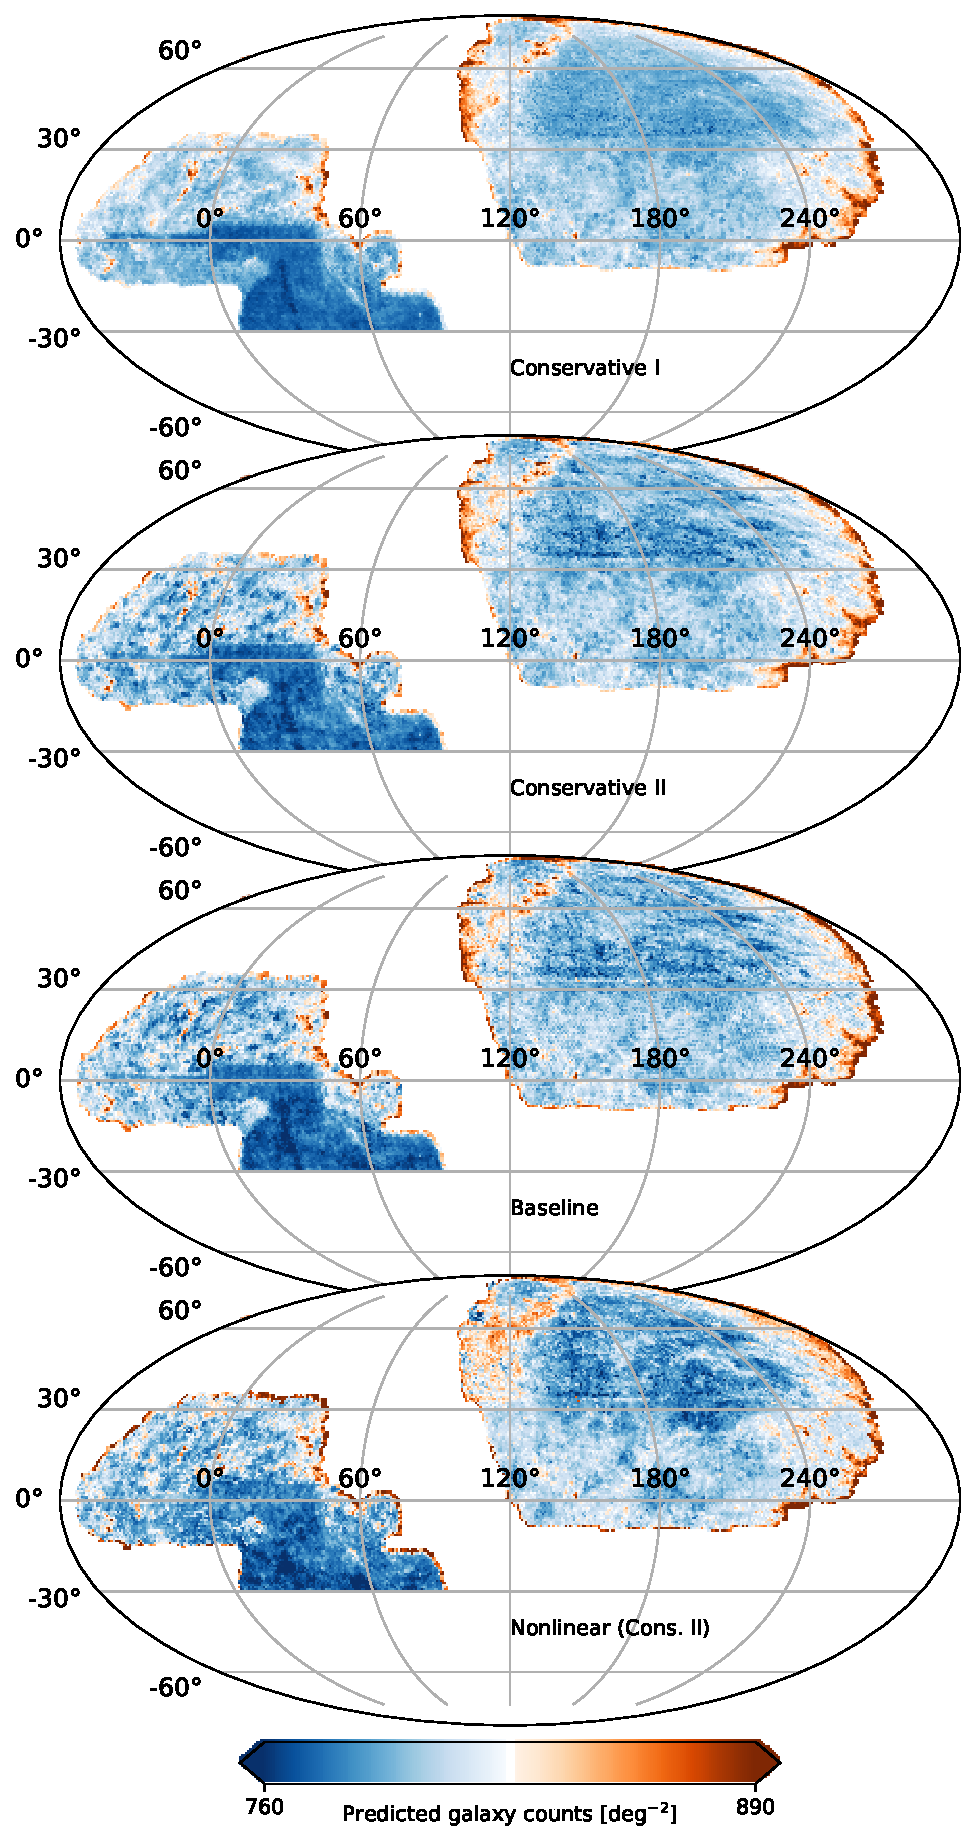
\includegraphics[width=0.45\textwidth]{figures/npred.pdf}
    \caption{Predicted galaxy counts from template regression. Baseline approach uses imaging maps from Zhou et al. (2022): EBV, galaxy depth in rgz, psfdepth in W1, and psfsize in grz. Conservative I uses EBV and galaxy depth in z, and Conservative II uses EBV, galaxy depth in z, and psfsize in r. In all approaches, the models are regressed on BASS+MzLS, DECaLS North, and DECaLS South separately.}
    \label{fig:npred}
\end{figure}



\begin{figure}
    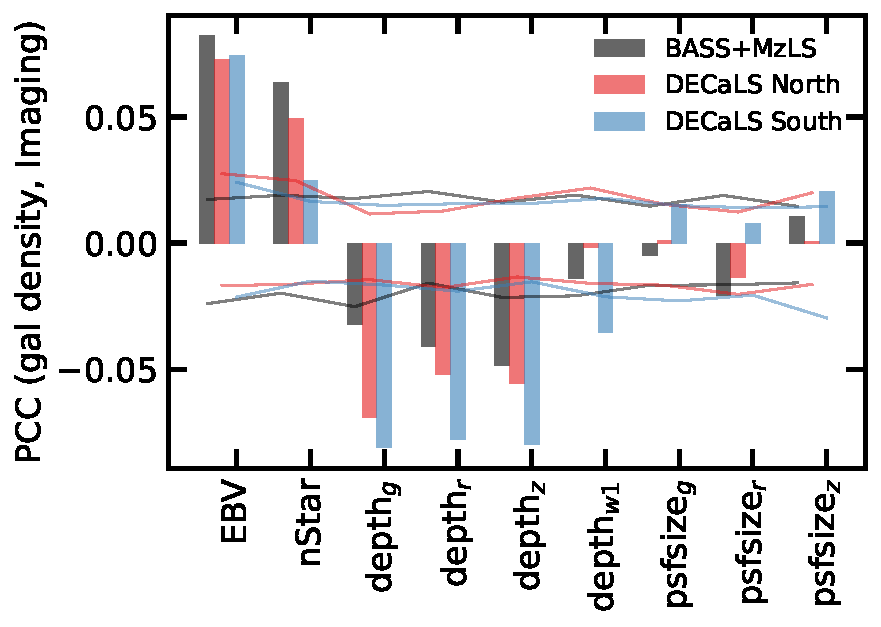
\includegraphics[width=0.45\textwidth]{figures/pcc.pdf} 
    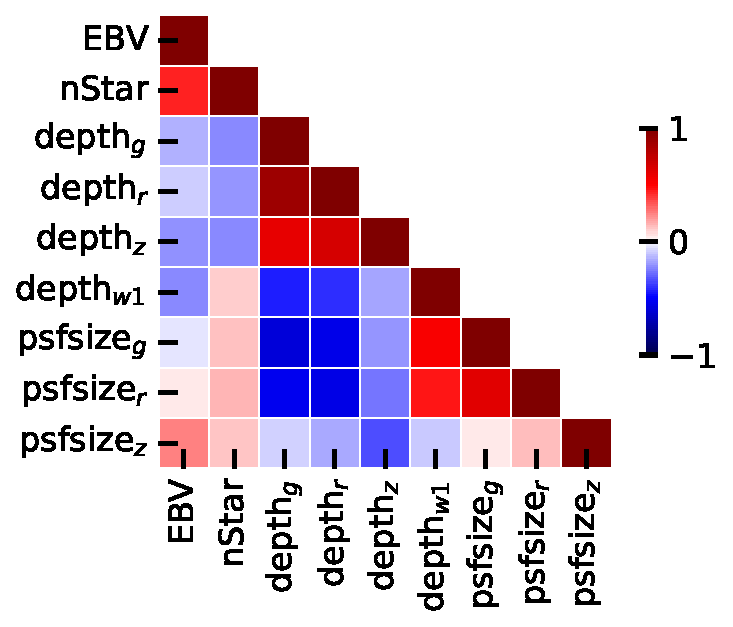
\includegraphics[width=0.45\textwidth]{figures/pccx.pdf}     
    \caption{Top: Spearman correlation coefficient between galaxy density and imaging properties. Solid curves represent the range of correlations observed in the mocks. Bottom: Pearson correlation coefficient between imaging properties.}
    \label{fig:pcc}
\end{figure}






\begin{table*}
  \begin{center}
    \caption{Selection criteria for the LRG targets.}
    \label{tab:ts}
    \begin{tabular}{lc}
    \hline
      \textbf{Criterion} &\textbf{Description}\\
      \hline   
     \textbf{DECaLS} & \\ 
     $z_{\rm fiber} < 21.7$  & faint limit  \\
     $z - W1 > 0.8 \times (r - z) - 0.6$ & Stellar rejection  \\
     $[(g-r >1.3)~{\rm AND}~((g-r) > -1.55*(r-W1) + 3.13)]~{\rm OR}~(r -W 1 > 1.8)$ & Remove low-z galaxies \\
     $[(r-W1 > (W1 - 17.26)*1.8)~{\rm AND}~(r - W1 > W1 - 16.36)]~{\rm OR}~(r-W1 > 3.29)$ & Luminosity cut \\ 
    \hline
     \textbf{BASS+MzLS} & \\ 
     $z_{\rm fiber} < 21.71$  & faint limit  \\
     $z - W1 > 0.8 \times (r - z) - 0.6$ & Stellar rejection  \\
     $[(g-r >1.34)~{\rm AND}~((g-r) > -1.55*(r-W1) + 3.23)]~{\rm OR}~(r -W 1 > 1.8)$ & Remove low-z galaxies \\
     $[(r-W1 > (W1 - 17.24)*1.83)~{\rm AND}~(r - W1 > W1 - 16.33)]~{\rm OR}~(r-W1 > 3.39)$ & Luminosity cut \\ 
      \hline
      \end{tabular}
  \end{center}
\end{table*}


\clearpage